\documentclass[a4paper, 11pt, landscape]{article}

\usepackage{mathptmx} % more compact font
\usepackage{amsmath}
\usepackage{amsfonts}
\usepackage{mathtools}
\usepackage{multicol}
\usepackage{enumitem}
\usepackage{paralist} % for compacter lists
\usepackage{hyperref} % for Todo's and similar things
\usepackage[left=4.5mm, right=4.5mm, top=4.5mm, bottom=6mm, landscape, nohead, nofoot]{geometry}
\usepackage[small,compact]{titlesec}
\usepackage[usenames,dvipsnames,svgnames,table]{xcolor}
\usepackage{xparse}
\usepackage{graphicx}
\graphicspath{ {./} }

% compact text
\linespread{0.9}
\setlength{\parindent}{0pt}

% compact lists even more
\setdefaultleftmargin{0em}{0em}{0em}{0em}{0em}{0em}

% compact sections
\titlespacing*{\section}{0pt}{0em}{0em}
\titlespacing*{\subsection}{0pt}{0em}{0em}
\titlespacing*{\subsubsection}{0pt}{0em}{0em}

% coloured section headings for easier read
\titleformat{name=\section}[block]
  {\sffamily}
  {}
  {0pt}
  {\colorsection}
\newcommand{\colorsection}[1]{%
	\colorbox{red!10}{\parbox[t][0em]{\dimexpr\columnwidth-2\fboxsep}{\thesection\ #1}}}


\titleformat{name=\subsection}[block]
  {\sffamily}
  {}
  {0pt}
  {\subcolorsection}
\newcommand{\subcolorsection}[1]{%
	\colorbox{orange!10}{\parbox[t][0em]{\dimexpr\columnwidth-2\fboxsep}{\thesubsection\ #1}}}


\titleformat{name=\subsubsection}[block]
  {\sffamily}
  {}
  {0pt}
  {\subsubcolorsection}
\newcommand{\subsubcolorsection}[1]{%
	\colorbox{blue!10}{\parbox[t][0em]{\dimexpr\columnwidth-2\fboxsep}{\thesubsubsection\ #1}}}
	
% environment for multicols inside a list
\NewDocumentEnvironment{listcols}{O{2} O{0pt}}
	{%
		\bgroup %
		\setlength{\multicolsep}{#2} %
		\begin{multicols*}{#1} %
	}
	{%
		\end{multicols*} %
		\egroup %
	}

% multicols lines & spacing
\setlength{\columnsep}{0.2cm}
\setlength{\columnseprule}{0.2pt}

% No page numbers
\pagenumbering{gobble}

% math helpers
\DeclareMathOperator*{\argmin}{arg\,min}
\DeclareMathOperator*{\argmax}{arg\,max}

\begin{document}
\begin{multicols*}{3}

\section{Probability Calculus}
$p(x|y)=\frac{p(x, y)}{p(y)}=\frac{p(x)p(y|x)}{\sum_{x}p(x)P(y|x)}=\frac{Prior \times Likelihood}{Evidence}$\newline
$p(x)=\sum\limits_{z}{p(x,z)}$\qquad
$p(x,y,z)=p(x)p(y|x)p(z|x,y)$\newline
$x \perp \!\!\!\!\! \perp y\ \Rightarrow\ p(x,y|z)=p(x|z)p(y|z)\ \wedge\ p(x|y,z)=p(x|z)$\newline
$E[kf(x)+ng(x)]=kE[f(x)]\cdot nE[g(x)]$\newline
$Cov(X)=E(X^2)-E(X)^2$ \qquad $Cov(aX+b)=a^2 Cov(X)$\newline
$E_{Y|X=x_i}[f(x_i,Y)]=\sum_{y'\in Y}f(x_i,y')p(y'|x_i,\theta)$

\section{Semirings $R=(A,\oplus,\otimes,\bar{0},\bar{1})$}
\subsection{$(A,\oplus,\bar{0})$ is a commutative monoid}
$(a\oplus b)\oplus c = a\oplus (b\oplus c)$
$\bar{0}\oplus a = a \oplus \bar{0} = a$
$a\oplus b = b \oplus a$

\subsection{$(A,\otimes,\bar{1})$ is a monoid}
$(a\otimes b)\otimes c = a \otimes (b \otimes c)$ \phantom{2. }$\bar{1}\otimes a = a \otimes \bar{1} = a$

\subsection{$\otimes$ distributes over $\oplus$: for all $a,b,c$ in $A$} 
$(a \oplus b)\otimes c = (a \otimes c) \oplus (b \otimes c)$ \newline
$c \otimes (a \oplus b) = (c \otimes a) \oplus (c \otimes b)$

\subsection{$\bar{0}\otimes a = a\otimes \bar{0}=\bar{0}$}
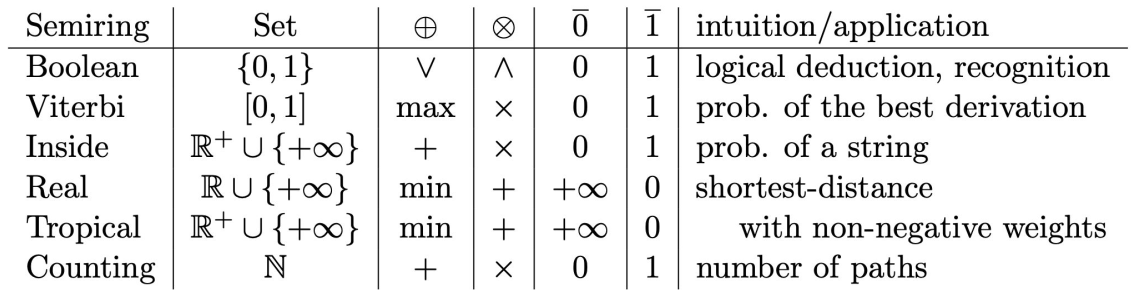
\includegraphics[scale=0.4]{semirings}
\textbf{Real for log-probabilities}: $\langle\mathbb{R}\cup\{-\infty\},max,+,-\infty,0\rangle$\newline
\textbf{Real for max-probabilities CKY}:$\langle\mathbb{R}^+,max,\times,0,1\rangle$\newline
\textbf{Real for LogSumExp}:$\langle\mathbb{R}\cup-\infty,log_+,+,-\infty,0\rangle$

\section{Backpropagation (Chainrule, DP)}
$\frac{\partial f}{\partial g}=\frac{\partial f}{\partial h}\cdot \frac{\partial h}{\partial g}$\quad
$\frac{\partial f_k}{\partial g_i}=\sum_{j=1}^{m}{\frac{\partial f_k}{\partial h_j}\cdot \frac{\partial h_j}{\partial g_i}}$\newline
\textbf{Constr. Th.}: Same asympt. complexity as the orig. func.

\section{Log-Linear Modeling (Softmax'd dotproduct)}
$p(y|x)=\frac{count(x,y)}{count(x)}$\qquad 
$p(y|x,\theta)=\frac{exp(\theta \cdot f(x,y))}{\sum_{y'\in Y}{exp(\theta \cdot f(x,y'))}}$\newline
\textbf{Binary}: $p(y|x,\theta)=\sigma(\theta\cdot x)=1/(1+exp(-\theta\cdot x))$\newline
$\theta_{MLE}=\underset{{\theta \in \Theta}}{argmax}\ L(\theta)$\qquad
$L(\theta)=\prod_{n=1}^{N}p(y_n|x_n,\theta)$\newline
$LL(\theta)=\sum_{n=1}^{N}log \ p(y_n|x_n,\theta)$\qquad $NLL(\theta)=-LL(\theta)$\newline
$\frac{\partial NLL(\theta)}{\partial\theta_k}=\underset{{observed}}{-\sum_{n=1}^{N}{f_k(x_n,y_n)}}+\underset{{expected}}{\sum_{n=1}^{N}{\sum_{y'\in Y}{p(y'|x_n,\theta)f_k(x_n,y')}}}$\newline
\textbf{Expectation matching}: observed = expected\newline
\textbf{Hessian}: $\nabla^2NLL(\theta)=\sum_{i=1}^{n}{Cov(f(x_i,Y))}$\newline
\textbf{Softmax}$(h,y,T)=\frac{exp(h_y/T)}{\sum_{y'\in Y}{exp(h_{y'}/T)}}, \ \ h_y=\theta \cdot f(x,y)$\newline
$T\rightarrow \infty$: uniform, max entropy\newline
$T\rightarrow 0$: annealing, max function, minimum entropy\newline
Softmax is diffbar for $T>0$\newline
\textbf{Exp. family}: $p(x|\theta)=\frac{1}{Z(\theta)}h(x)exp(\theta\cdot \phi(x))$\newline
finite sufficient stat., conjugate priors, max. entropy distr.
\textbf{Skip-Gram}: $p(c|w)=\frac{1}{Z(c)}exp(e_{wrd}(w)\cdot e_{ctx}(c))$


\subsection{Hessian Matrix}
\textbf{Jacobian $\nabla f(x)$}: $J_{ij}=\frac{\partial f_i}{\partial x_i}$\quad
\textbf{Hessian $\nabla^2 f(x)$}: $(H_f)_{ij}=\frac{\partial^2 f}{\partial x_i\partial x_j}$\newline
\textbf{Trick}: $e_i^T\nabla^2f(x)=\nabla(e_i^T\nabla f(x))$\newline
\textbf{Recursion}: $O(mn^{k-1})$

\section{Feed-forward NN: $\sigma(W_i^T\cdot ReLU(W_j^Tx+b_j)+b_i)$}
Non-linearity + learning the structure, feature engineering is tedious because we don't know the structure, thus feature extractor (architecture) engineering\newline
Will not learn if weights are all initialized $0$ or the same.\newline
\textbf{Finite-difference procedure}: \newline
$O((((n+1)\cdot k_1+(\sum_{l=1}^{L-1}(k_l+1)\cdot k_{l+1})+(k_L+1)\cdot c)^2)$

\subsection{Activation Function (non-linearities)}
$\sigma(x)=1/(1+exp(-x))$\quad
$\sigma'(x)=\sigma(x)(1-\sigma(x))$\newline
$tanh(x)=2\sigma(2x)-1$\quad
$tanh'(x)=1-tanh^2(x)=1/(x^2+1)$\newline
$ReLU(x)=max(0,x)$, PReLU, ELU, SELU, SoftPlus\newline
\textbf{Dead neurons}: ReLU with $x<0\rightarrow$ PReLU, Leaky ReLU

\subsection{Vanishing Gradient}
High (absolute) input values (sigmoid, tanh, RNN) $\rightarrow$ partial derivatives $\sim 0$ $\rightarrow$ abs(weights) $\ll 1$ $\rightarrow$ model stops learning eventually.\newline
\textbf{Solution}: ReLU, LSRM, GRU, fewer layers, batch norm

\subsection{Exploding Gradient}
Large increase in the norm of the gradient during training (NN, RNN). All gradients $> 1\rightarrow$ large updates $\rightarrow$ overflow.\newline
\textbf{Solution}: fewer layers, regularization

\section{RNN}
$h_t=f(x_t, h_{t-1})$, with cell $f$ (RNN, GRU, LSTM)\newline
$\frac{\partial h_{m+k}}{\partial h_m}=\prod_{i=0}^{k-1}\frac{\partial h_{m-i}}{\partial h_{m-i-1}}$\newline
\textbf{RNN}: $h_t=tanh(\theta h_{t-1}+x_t)$ (or $\sigma()$)\newline
GRU tries to solve the vanishing/exploding gradient problem.

\section{Language Modeling}
\textbf{Preprocessing}: Tokenization, Lower casing, Stemming, Stop word removal, reducing vocabuulary\newline
\textbf{Features}: n-grams, one-hot-encoding, bag-of-words, word embedding, bag of embeddings\newline
\textbf{Locally normalized}: $Z=\sum_{y'\in V^*}\prod_{t=1}^{|y'|}{\theta_{y'_{\le t}}=1}$\newline
\textbf{Globally normalized}: Floyd-Warshall-Kleene, MEMM

\subsection{n-gram}
$p(y_t|y_{<t})=p(y_t|y_{t-1},...,y_{t-n+1})=$ softmax$(h_{y_t})$\newline
\textbf{Trade-off}: small $n \rightarrow$ high bias\qquad
big $n \rightarrow$ high variance\newline
\textbf{States}: $m+|V|^{n-1}+1$, $m=|V|^{n-2,\;n>1}$ or $0$\qquad $O(|V|^{n-1})$\newline
\textbf{Bengio et al. 2003}: Language model as neural network, use e word embeddings in MLP, using neural parametrization of an n-gram model\newline
$h=b_1+W_1\cdot e(hist)+W_2\cdot tanh(b_2+W_3\cdot e(hist))$

\section{Conditional Random Fields (CRFs) (locally normalized)}
\textbf{Part-of-speech (POS) tagging}: Adj., Nouns, Verbs, etc.\newline
Use graph for score$(<D,N,V,N>,w)$\newline
$p(t|w)=\frac{exp(score(t,w))}{\sum_{t'\in T}exp(score(t',w))}$\newline
score$(t,w)=\sigma\cdot f(t,w)$ or $=NN_{\sigma}(t,w)$\newline
\textbf{Structure assumption}: $p(t|w)=\frac{exp(\sum_{n=1}^N score(\langle t_{n-1},t_n \rangle,w))}{\sum_{t'\in T^N} exp(\sum_{n=1}^N score(\langle t'_{n-1},t'_n \rangle,w))}$\newline
$LL(\theta)=\sum_{i=1}^{I}{score(t^{(i)},w^{(i)}))-T\;log\sum_{t'\in T^N}exp\frac{score(t',w^{(i)})}{T}}$\newline
\textbf{For $T\rightarrow 0$}: Viterbi (structured perceptron)

\subsection{Computing the normalizer (DP)}
$\beta(w,t_N)\leftarrow 1$\newline
\textbf{for }$n\leftarrow N-1,...,0:$\newline
\phantom{for }$\beta(w,t_n)\leftarrow \oplus\; exp(score(\langle t_n,t_{n+1}\rangle,w))\otimes\beta(w,t_{n+1})$\newline
\textbf{Complexity}: $O(|tagset|^{'n\;\text{of n-grams}'}|sentence|)$

\section{Constituency Parsing}
\subsection{Context-free grammar: $G=\langle N,S,\Sigma,R\rangle$}
Rules can be applied to a non-terminal regardless of context.\newline
$N\;-$ set of nonterminal symbols\newline
$S\;-$ start symbol\newline
$\Sigma\;-$ set of terminal symbols\newline
$R\;-$ set of production rules\newline
\textbf{Problem}: I like to play bridge and bob chess $\rightarrow$ cross-serial dependency does not work

\subsection{Chomsky normal form: $(N_1\rightarrow N_2 N_3)$ and $(N\rightarrow a)$}

\subsection{Probabilistic CFG} 
Sum over a rule $= 1$, locally normalized, probability will be multiplied over tree

\subsection{Weighted CFG}
Non-negative, globally normalized, weight will be $exp()$ multiplied over tree, structured softmax\newline
$p(t)$ is infinite, $p(t|s)$ finite if no cycles (CNF)!\newline
$p(t|s)=\frac{\prod_{r\in t}exp(score(r)}{\sum_{t'\in T(s)}\prod_{r'\in t'}exp(score(r'))}$\newline

\subsection{CKY $O(N^3|R|)$}
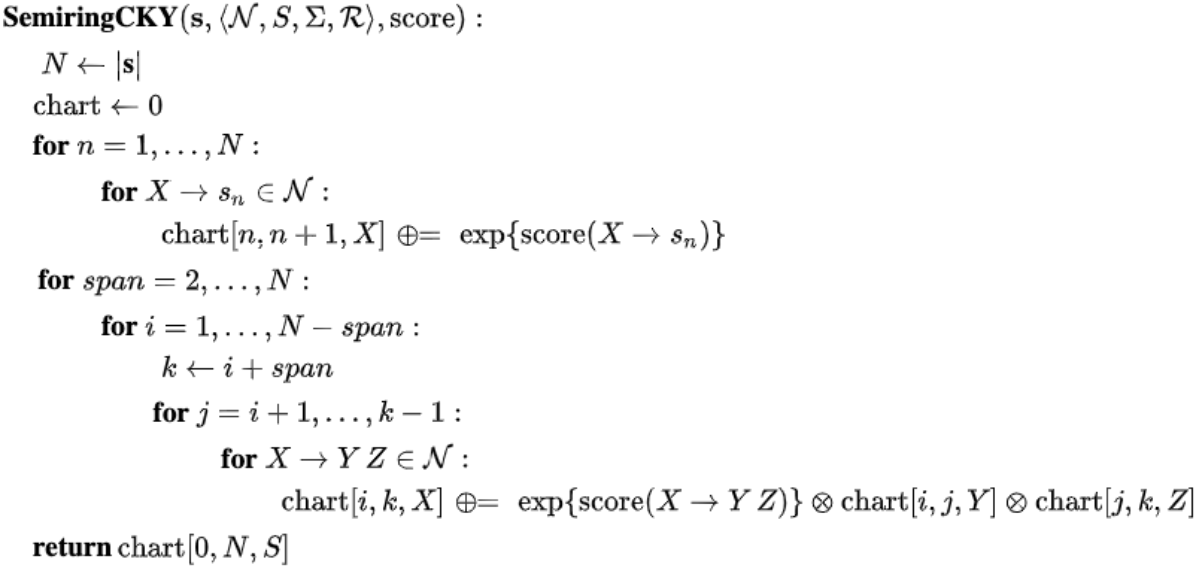
\includegraphics[scale=0.37]{cky}

\section{Dependency Parsing}
\textbf{Dependency Tree $=$ Directed Spanning Tree}\newline
All non-root nodes have one incoming edge, no cycles, only one outgoing from root\newline
\textbf{Projective dependency trees}: no crossings, close to constituency, use cky \newline
\textbf{Non-projective dependency trees}: crossings, close to discontinued constituents, $n^{n-2}$ Spanning trees, $(n-1)^{n-2}$ root constraints $\rightarrow O(n^n)$\newline
\textbf{Matrix-Tree Theorem}: 
$L_{ij}=\overset{{i\ne j}}{-A_{ij}}\;\;|\;\;
\overset{{i=j}}{(\rho_j+)\sum_{k\ne i} A_{kj}}\;\;|\;\;
\overset{{i=1}}{\rho_{j}}$\newline
$p(t|w)=\frac{\prod_{(i\rightarrow j)\in t}exp(score(i,j,w))}{|L|}\rightarrow O(n^3)$\newline
\subsection{Chu-Liu Edmonds Algoritm $O(n^2)$}
1. Greedy selection (best incoming for each node, except root)\newline
2. On cycle $\rightarrow$ contract (cycle through mult. incoming, sum)\newline
3. For mult. root, find replacement with lowest swap cost

\section{Lambda Calculus (Free and Bound)}
\textbf{Appl.}: $M\;N\;P \equiv ((M\;N)\;P)$\quad
\textbf{Abstr.}: $\lambda x.M\;N\equiv \lambda x.(M\;N)$\newline
$A\rightarrow B \equiv \neg A \vee  B \equiv \neg(A \wedge \neg B)$\quad
\textbf{$\alpha$-conversion}: $\lambda x.x\;\rightarrow \lambda y.y$\newline
\textbf{$\beta$-reduction}: $\lambda x.x\;z \rightarrow z$\qquad
\textbf{$I$-combinator}: $\forall x:\;(I\;x)=x$\newline
\textbf{$K$-combinator}: $\forall x,y:\;(K\;x\;y)=((K\;x)y)=x$\quad
$(S\;K\;K)\equiv I$\newline
\textbf{$S$-combinator}: $\forall x,y,z:\;(S\;x\;y\;z)=(x\;y(y\;z))=((x\;z)(y\;z))$
\textbf{$B$-combinator}: $\forall x,y,z:\;(B\;x\;y\;z)=(x(y\;z))$\newline
\textbf{$C$-combinator}: $\forall x,y,z:\;(C\;x\;y\;z)=((x\;z)y)$\newline
\textbf{$T$-combinator}: $\forall x,y:\;(T\;x\;y)=(y\;x)$

\section{Weighted Finite-State Transducers (WFST)}
\textbf{Transliteration}: map to another character set (alphabet)\newline
$T=\langle Q,\Sigma,\Omega,\lambda,\rho,\delta\rangle$\newline
$Q$: all states (finite set)\newline
$\Sigma$: input vocabulary \newline 
$\Omega$: output vocabulary\newline
$\lambda$: function map to init scores\newline
$\rho$: function map to final scores\newline
$\delta$: transition function, mapping transitions (arcs) to scores\newline
$Z=\alpha^T\left(\sum_{\omega\in\Omega\cup{\epsilon}}{W^{(\omega)}}\right)^*\beta$\newline
$\sum_{i=1}^{I}{log\;p(y^{(i)}|x^{(i)})}=\sum_{i=1}^{I}{score(y^{(i)},x^{(i)})-log\;Z(x^{(i)})}$\newline
\subsection{Floyd-Warshall-Kleene Algorithm $O(n^3)$}
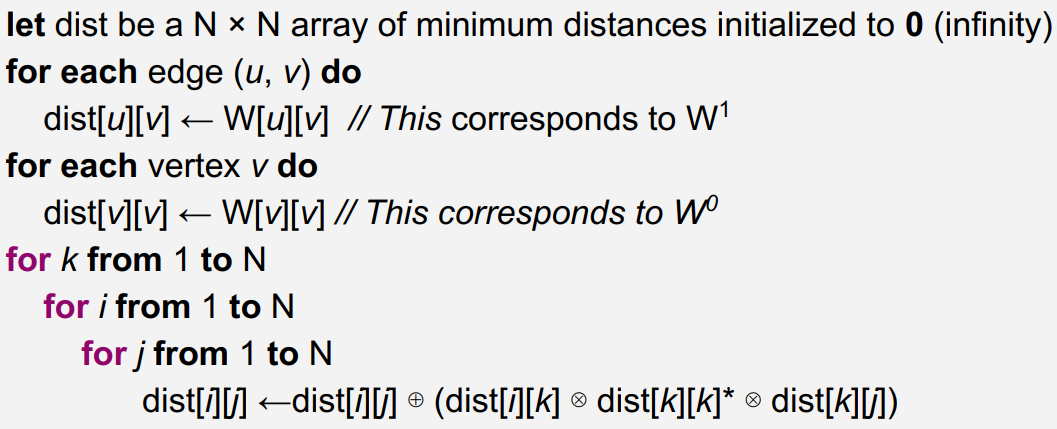
\includegraphics[scale=0.42]{fwk}

\section{Sequence-to-Sequence Models}
$z=encoder(x)$\qquad$y\;|\;x\sim decoder(z)$\newline
\textbf{Enc}: $\underset{{\theta}}{argmax}\sum_{i=1}^{N}{log\;p(y^{(i)}|x^{(i)}},\theta)$\newline$=\underset{{\theta}}{argmax}\sum_{i=1}^{N}\sum_{t=1}^{|y^{(i)}|}{log\;p(y_t^{(i)}|x^{(i)},y_{<t}^{(i)},\theta)}$\newline
\textbf{Dec}: $score:=log\;p(y|x)=\sum_{t=1}^{|y|}{log\;p(y_t|x,\langle y_{t-n},...,y_{t-1}\rangle)}$\newline
For one $y$: $O(|\Sigma|\cdot n_{max})$, for all $y$: $O(|\Sigma|^{n_{max}})$\newline
$\rightarrow$ beam search, sampling, greedy search\newline
Only last hidden state of seq. is passed to decoder!\newline
\textbf{Used for}: mach. transl., text summarization, img captioning

\subsection{Attention Mechanism}
\textbf{RNN+NN}: RNN gets $h_{t-1}$ \& previous NN output, NN gets $h_t$ and attention vector (all $h_i$ of enc, weighted with softmax, done for each dec step)\newline
\textbf{Weights}: $\alpha^{(t)}=softmax(score(q_t,K))$\newline
\textbf{Context}: $c^{(t)}=\alpha^{(t)T}V$\newline
\textbf{Vec rep (hid. state) produced by enc at pos i}: $k_i=v_i=h_i^{(e)}$\newline
\textbf{Vec rep produced by dec at pos $t$}: $q_t=h_t^{(d)}$\newline
\textbf{= stacked encoder vector representations}: $K=V=H^{(e)}$

\section{Axes of Modeling}
\subsection{Probabilistic models}
Prob. distr. over classes (outcomes)\newline
\phantom{..}\textbf{+} probability theory, convenient \& intuitive framework\newline 
\phantom{..}\textbf{-} assump. about distr. (indep./distr. of noise) may be false\newline
\textbf{Discriminative}: models decision boundary (CRF, RNN)\newline
\textbf{Generative}: models distr. of class (n-gram, MRF, RNN)\newline
\phantom{....}\textbf{Structured predictors}: Use if decomposing output space\newline
\phantom{....}is helpful (output space is too big)\newline
\phantom{........}\textbf{Locally Normalized}: + efficient to train, only prediction\newline
\phantom{........}of current state, - label bias (n-gram, RNN)\newline
\phantom{........}\textbf{Globally Normalized}: + scores at each time step can\newline
\phantom{........}have diff. importance, - comp. global norm. constant\newline
\phantom{........}structural indep. assump. are crit. (CRF, MRF, RNN)

\subsection{Non-probabilistic models}
Separate feature space and return the class associated with the space where they believe a sample comes from\newline
\phantom{..}\textbf{+} more interpretable\newline 
\phantom{..}\textbf{-} no direct way to quantify uncertainty of a prediction\newline
\textbf{Learned}: Perceptron, SVM\newline
\textbf{Manually-crafted}: CFG, LIG

\subsection{Bias/Variance Trade-off}
A biased simpler model can have better overall performance than a complicated
unbiased model (due to lower variance of the simpler model)

\subsection{Loss-Function}
Convexity, continuity, diffbar, comp. complexity, sensitive to noise and outliers, connection to end goal, tradeoff between classes\newline
\textit{cross-entropy loss func. $\equiv$ negative log-likelihood of
model}\newline
\textbf{MLE}: efficient to evaluate, consistent, asympt. efficient, only for probabilistic models, can easily overfit (bad on unseen)\newline
\textbf{Alternatives}: Maximum margin (hinge), logistic, exponential

\subsection{Regularization (improve Generalization)}
Adding prior information to prevent overfitting to noise\newline
\textbf{Deep Learning}: Weight Decay, Dropout, Early Stopping, Batch normalization \newline
\textbf{Lasso L1}: $L(\theta)+\lambda||\theta||_1$, encourages many coeff to exactly zero, not diffbar\newline
\textbf{Ridge L2}: $L(\theta)+\lambda||\theta||_2^2$, shrinks params to small non-zero values\newline
\textbf{Interpretation $\theta\sim\mathcal{N}(0,\tau^2I)$}: $\tau^2$ is a measure of confidence in our prior; the lower $\tau^2$, the more ”belief” we
place in our prior relative to the data. Since in the case of ridge, our prior mean is zero, this means that the lower we choose $\tau^2$ the stronger we bias our resulting coefficients toward the prior mean (i.e., zero). Thus, since $\sigma^2$ is fixed, the lower we choose $\tau^2$ the stronger the regularization and vice versa (i.e., high $\tau^2$ implies little confidence in our prior and thus low regularization).

\raggedcolumns
\end{multicols*}
\end{document}
